\section{Prospects for future e-learning projects on \ac{fiit} \label{sec:fiit_prospects}}

% As already mentioned in (Section~\ref{sec:engagement})

A part of the evaluation is determining the students' interest in e-learning materials at \ac{fiit} and assessing the usefulness of conducting further research in the topic. 

The feedback questionnaire displays an enthusiastic approach towards e-learning materials, especially in the \ac{pv} group. That is further reinforced by textual responses (see Section~\ref{sec:text_feedback}) to its open-ended questions.

The \ac{pv} group expressed more interest in e-learning, as well as a very high (8+) interest in encountering more non-neutral study materials. Average general satisfaction with the courses is also higher in \ac{pv} than in \ac{cv}, though high in the combined measurements as well. 

Both groups agreed that the courses added value to the subject they were asked to fill out the course in, and that it helped them improve their understanding of the \ac{uml} class diagram in roughly equal measure.

Responses to \enquote{I would voluntarily take a similar course} show less conviction - the students might only take such courses if offered extra credits for doing so or if it were mandatory. Another interpretation of the question results are that they would voluntarily take a course - if it were better designed.

\FloatBarrier
\begin{figure}[ht]
\centering
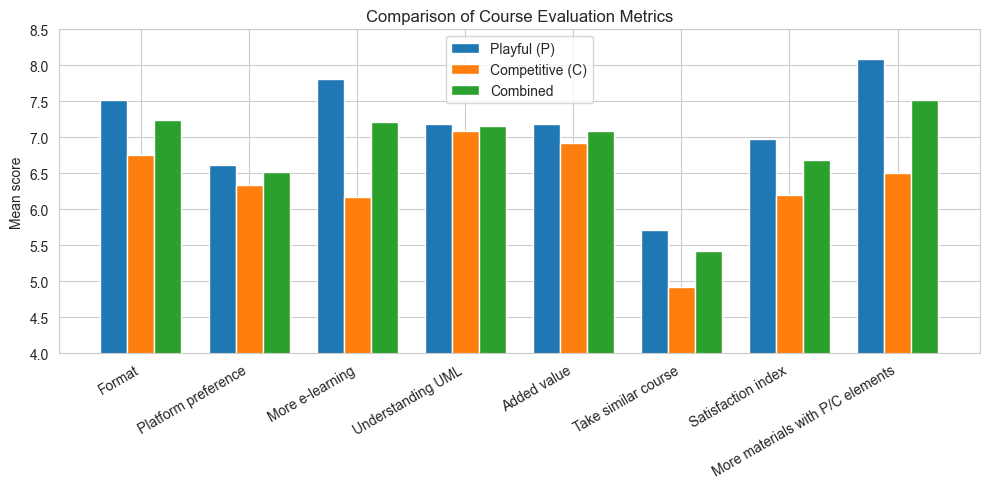
\includegraphics[width=1\textwidth]{assets/images/eval/engagement/prospects_for_elearning.png}
\caption{Students' opinions on e-learning at \ac{fiit}}
\label{fig:prospects_for_elearning}
\end{figure}
\FloatBarrier

Full metric names in respective order:
\begin{itemize}
    \item I enjoyed the format of the course.
    \item If there are other courses, I would not mind them being made using the same platform as this one (Moodle).
    \item I would like to encounter more e-learning materials during my studies at FIIT STU.
    \item This course helped me develop a better understanding of the UML class diagram.
    \item This e-learning material added value to the university course PSI.
    \item I would voluntarily take a similar course.
    \item satisfaction\_index (see Section~\ref{sec:data_prep} for calculation)
    \item I want to encounter more study materials with playful/competitive elements
\end{itemize}

% \textbf{Summary}

% Students expressed general interest in e-learning materials and their use at \ac{fiit}. The reception of this course suggests further experiments on the topic of e-learning at \ac{fiit} should be conducted with a preference for playfulness over competition. 

% It should be noted that the difference in overall satisfaction with the course as well as interest in e-learning in general might be at least partially attributed to a better design of \ac{pv} compared to \ac{cv}. However, there is no way to verify the assumption without further experiments.